\documentclass[14pt,letterpaper]{article}
\usepackage[utf8]{inputenc}
\usepackage[spanish]{babel}
\usepackage{times}
\usepackage[left=3cm,top=2.5cm,bottom=2.5cm,right=2.5cm]{geometry}
\usepackage{graphicx}
\author{Perez de Alba Santiago Eduardo.}

\begin{document}
\begin{center}

\LARGE \textbf{Universidad Politécnica de la Zona Metropoilitana de Guadalajara\\}


\includegraphics[scale=1]{Upzmg.png} 

\large \textbf{2\_ 6\_ Construir\_ un\_ amplificación\_ con\_ conexión\_ Darlington.}

\end{center}

\vspace{1cm} 
\large \textbf{Nombre: \\Perez de Alba Santiago Eduardo.\\ Romero Jauregui Osvaldo\\
\vspace{0.5cm} Carrera: Ingeniería en Mecatronica.\\
\vspace{0.5cm} Materia: Sistemas Electrónicos de Interfaz.\\
\vspace{0.5cm} Curso: Septiembre-Noviembre del 2019.\\
\vspace{0.5cm} Docente: Moran Garabito Carlos Enrique.}\\
\vspace{0.5cm}
\small \textbf{07 de Diciembre del 2019}


\newpage
\section{Introducción:}
\
Durante la elaboración de esta practica se pudo retomar conocimientos básicos sobre la aplicación de los relevadores, los transistores 2n2222, e incluiremos nuevos conceptos como el de los Fotoresistor o LDR, como es que funciona e información respecto al mismo, utilizaremos un Contactor industrial para denotar el funcionamiento del mismo.

\section{Objetivo:}
\begin{itemize}
\item El objetivo de esta práctica, es el conocer la correcta utilización de nuestro transistor Darlington, (en su defecto 2 de nuestros transistores 2n2222) para así poder manejar el aumento de la potencia, requerido para la correcta activación de nuestro Relay.
\item El objetivo principal de esta segunda parte de la practica es el hacer las conexiones correctas de nuestro fotoresistor (LDR).
\end{itemize}
\section{Materiales:}
\begin{itemize}
\item Fotoresistor (LDR)
\item Optoacopladores
\item Relays
\item Push buttons
\item Jumpers (macho-macho)
\item Transistor Darlington (2 transistores 2n2222 en su defecto)
\item Diodo
\item Diodo Led
\item Fuente de voltaje
\end{itemize}
\section{Marco teórico:}
Un LDR es un resistor que varía su valor de resistencia eléctrica dependiendo de la cantidad de luz que incide sobre él. Se le llama, también, fotorresistor o fotorresistencia. El valor de resistencia eléctrica de un LDR es bajo cuando hay luz incidiendo en él (en algunos casos puede descender a tan bajo como 50 ohms) y muy alto cuando está a oscuras (puede ser de varios megaohms).

Los LDR se fabrican con un cristal semiconductor fotosensible como el sulfuro de cadmio (CdS). Esta celdas son sensibles a un rango amplio de frecuencias lumínicas, desde la luz infrarroja, pasando por la luz visible, y hasta la ultravioleta.

La variación de valor resistivo de un LDR tiene cierto retardo, que es diferente si se pasa de oscuro a iluminado o de iluminado a oscuro.

Por esta razón un LDR no se puede utilizar algunas aplicaciones, en especial en aquellas en que la señal luminosa varía con rapidez. El tiempo de respuesta típico de un LDR está en el orden de una décima de segundo.

La lentitud relativa del cambio es una ventaja en algunos casos, porque así se filtran variaciones rápidas de iluminación que podrían hacer inestable un sensor (por ejemplo cuando está iluminado por un tubo fluorescente alimentado por corriente alterna), En otras aplicaciones (como la detección de luminosidad para saber si es de día o es de noche) la lentitud de la detección no es importante.

Contactor Industrial
El contactor eléctrico es  un dispositivo capaz de permitir o bloquear el paso de la corriente, a través de la apertura o cierre de sus contactos,este dispositivo tiene la posibilidad de ser activado según su tipo de clasificación, Los contactores pueden ser clasificados por diferentes sistemas ya sea por su constitución, por su tipo de contactos, por corriente, etc. A continuación les dejaremos algunos de los tipos de clasificaciones.

\section{Desarrollo:}
1)	Iniciamos nuestro circuito usando como base los circuitos anteriores, parte de este lo conectamos de la siguiente manera:
\
\begin{figure}[h!]
\begin{center}
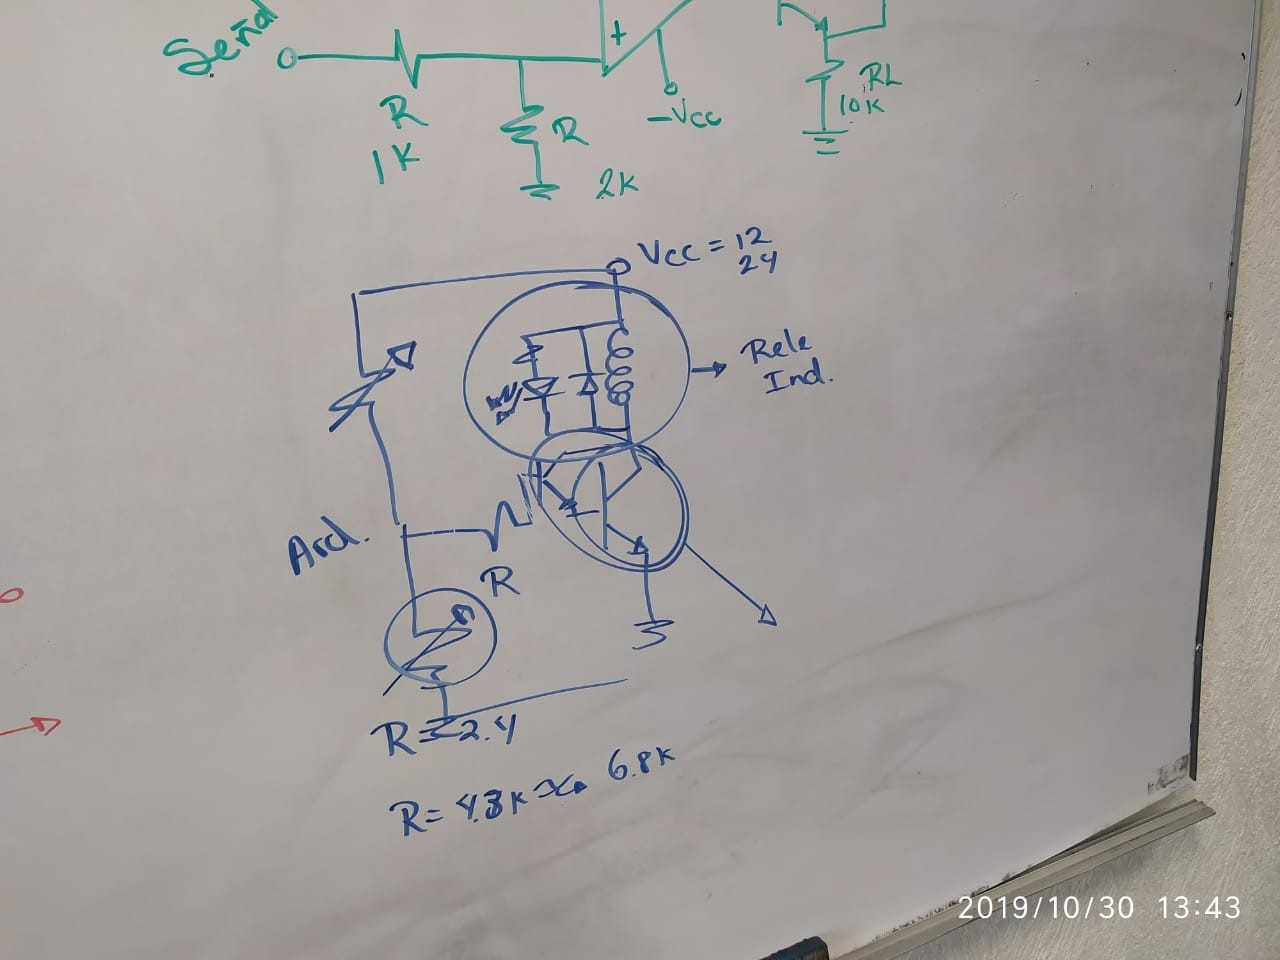
\includegraphics[scale=0.2]{EsquemaDarlington.jpg}  
\caption{Esquema de Darlington.}
\end{center}
\end{figure}

\newpage
2)	Al tener nuestras conexiones realizadas conforme a nuestra practica 2  (Optoacopladores) se sustituye el relevador que se activa junto a colector a una de las patas del embobinado, y colocamos nuestro contactor industrial.
\
\begin{figure}[h!]
\begin{center}
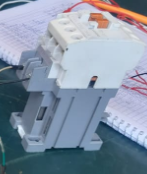
\includegraphics[scale=1]{ContactorIndustrial.png} 
\caption{Contactor Industrial.}
\end{center}
\end{figure}



\section{Resultados:}
Como era de esperarse, nuestro resultado final fue la correcta activación de nuestro contactor, utilizando el voltaje necesario para esto (24 v).
\
\begin{figure}[h!]
\begin{center}
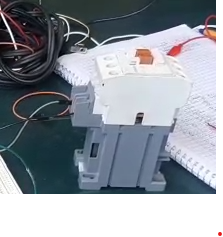
\includegraphics[scale=0.5]{ContactorIndustrial1.png}
\caption{Resultado} 
\end{center}
\end{figure}

\
\begin{figure}[h!]
\begin{center}
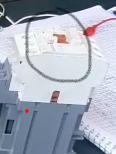
\includegraphics[scale=1]{ContactorIndustrial2.png}
\caption{Resultado}
\end{center}
\end{figure}

\section{Conclusión:}
\begin{itemize}
\item Durante el desarrollo de la practica se pudo comprender el funcionamiento del LDR o del Foto-resistor mediante el cual lográbamos realizar el cambio en el contactor una vez que reducía la luz que recibía el foto-resistor, mientras que cuando aumentaba la luminosidad recibida comenzaba a aumentar el contactor se apagaba (hacia el cambio).
\item Mientras se realizaba la practica se encontraron con varios inconvenientes al principio, ya que no se encontraba el Contactor industrial por lo tanto se utilizo un relay temporal, con el cual se comprobó el correcto funcionamiento de nuestro circuito, una vez encontramos nuestro Contactor se pudo reemplazar y probar nuevamente, obteniendo el resultado esperado.
\end{itemize}

\end{document}